\chapter{Appendix}
\label{c:appendix}
Note that the speed of light, the particle mass, and the Boltzmann constant are set to unity in Appendix for simplicity.
\definecolor{AppendixAf}{RGB}{186, 158, 54}
\definecolor{AppendixAfHot}{RGB}{214, 49, 34}
\definecolor{AppendixAfCold}{RGB}{103, 138, 235}
\definecolor{AppendixAfHori}{RGB}{57, 204, 113}

\section{Initial guess for Newton-Raphson iteration}
\label{The choice of initial guesses}
We use the Newton-Raphson iteration to find the root $\tilde{h}$ of Equation~(\ref{transcendental equation}). The iteration requires the derivative of \Cref{transcendental equation} with respect to $\tilde{h}$:
\begin{equation}
\frac{df}{d\tilde{h}}=2\tilde{h}+2-2T-2\left(\tilde{h}+1\right)\frac{dT}{d\tilde{h}}+\frac{2T\left(\tilde{h}+1\right)^4\frac{dT}{d\tilde{h}}+2T\left(\tilde{h}+1\right)\left(\frac{\abs{\mathbf{M}}}{D}\right)^2\left[\left(\tilde{h}+1\right)\frac{dT}{d\tilde{h}}+T\right]}{\left[\left(\tilde{h}+1\right)^2+\left(\frac{\abs{\mathbf{M}}}{D}\right)^2\right]^2},
\end{equation}
where
\begin{equation}
\frac{dT}{d\tilde{h}}=\frac{4\tilde{h}+4}{5\tilde{h}+5+\sqrt{9\tilde{h}^2+18\tilde{h}+25}}
-\frac{\left(2\tilde{h}^2+4\tilde{h}\right)\left(\frac{9\tilde{h}+9}{\sqrt{9\tilde{h}^2+18\tilde{h}+25}}+5\right)}{\left(5\tilde{h}+5+\sqrt{9\tilde{h}^2+18\tilde{h}+25}\right)^2},
\label{dT_dh}
\end{equation}
follows from \Cref{T of h}.

The root-finding iteration also requires an initial guess of $\tilde{h}_{\text{guess}}$, for which we suggest the following procedure. In the low-$T$ limit, we Taylor expand Equation (\ref{transcendental equation}) in powers of $\tilde{h}$ and keep the first- and second-order terms:
\begin{equation}
\left(\frac{\tilde{E}}{D}\right)^2+2\left(\frac{\tilde{E}}{D}\right)-\left(\frac{\abs{\mathbf{M}}}{D}\right)^2
=\frac{6}{5}\tilde{h}+\left\{\frac{43}{125}+\frac{4}{25\left[1+\left(\frac{\abs{\mathbf{M}}}{D}\right)^2\right]}\right\}\tilde{h}^2.
\label{cold limit of transcendental eq}
\end{equation}
Solving Equation~(\ref{cold limit of transcendental eq}) for the unknown $\tilde{h}$ gives the positive solution:
\begin{equation}
{\scriptstyle
\tilde{h}_{\text{guess}}
=\frac{
\sqrt{125\left[1+\left(\frac{\abs{\mathbf{M}}}{D}\right)^2\right]\left[43\left(\frac{\abs{\mathbf{M}}}{D}\right)^2+63\right]\left[\left(\frac{\tilde{E}}{D}\right)^2+2\left(\frac{\tilde{E}}{D}\right)-\left(\frac{\abs{\mathbf{M}}}{D}\right)^2\right]}}
{\left[43\left(\frac{\abs{\mathbf{M}}}{D}\right)^2+63\right]\left\{75\left[1+\left(\frac{\abs{\mathbf{M}}}{D}\right)^2\right]+\sqrt{125\left[1+\left(\frac{\abs{\mathbf{M}}}{D}\right)^2\right]\left[43\left(\frac{\abs{\mathbf{M}}}{D}\right)^2+63\right]\left[\left(\frac{\tilde{E}}{D}\right)^2+2\left(\frac{\tilde{E}}{D}\right)-\left(\frac{\abs{\mathbf{M}}}{D}\right)^2\right]+75^2\left[1+\left(\frac{\abs{\mathbf{M}}}{D}\right)^2\right]^2}\right\}}.
}
\label{guess for cold fluid}
\end{equation} In the opposite high-$T$ limit, Equation~(\ref{transcendental equation}) can be reduced to
\begin{equation}
\left(\frac{\tilde{E}}{D}\right)^2+2\left(\frac{\tilde{E}}{D}\right)-\left(\frac{\abs{\mathbf{M}}}{D}\right)^2
=\frac{9}{16}\tilde{h}^2,
\label{hot limit of transcendental eq}
\end{equation}
which leads to
\begin{equation}
\tilde{h}_{\text{guess}}=
\frac{4}{3}\sqrt{\left(\frac{\tilde{E}}{D}\right)^2+2\left(\frac{\tilde{E}}{D}\right)-\left(\frac{\abs{\mathbf{M}}}{D}\right)^2}.
\label{guess for hot fluid}
\end{equation}
Equation~(\ref{guess for cold fluid}) and Equation~(\ref{guess for hot fluid}) provide two initial guesses for `cold' and `hot' gases, respectively. The threshold to distinguish between `cold' gases and `hot' gases is given by
\begin{equation}
\left\{\frac{1800\left[1+\left(\frac{\abs{\mathbf{M}}}{D}\right)^2\right]}{437\left(\frac{\abs{\mathbf{M}}}{D}\right)^2+117}\right\}^2,
\label{ColdHot}
\end{equation}
which is obtained by equating Equations (\ref{guess for cold fluid}) and (\ref{guess for hot fluid}) (see \Cref{fig:FunHTilde}). If $(\tilde{E}/D)^2+2(\tilde{E}/D)-\left(\abs{\mathbf{M}}/D\right)^2$ is greater than \Cref{ColdHot}, we choose Equation~(\ref{guess for hot fluid}) as an initial guess for the Newton-Raphson iteration (hot gases); otherwise, we choose \Cref{guess for cold fluid} (cold gases).
\begin{figure}
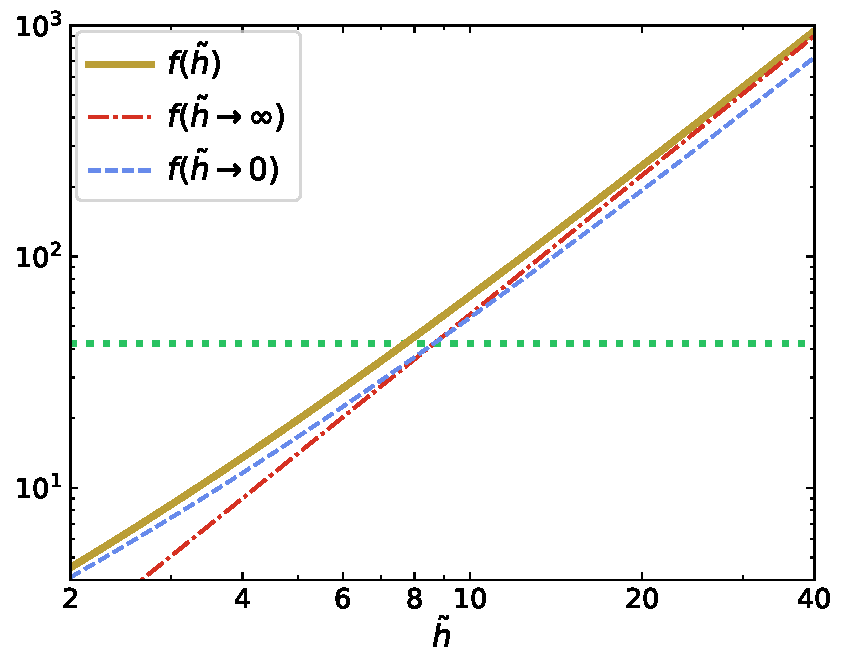
\includegraphics[scale=0.7]{figures/FunHTilde.pdf}
\caption{$f(\tilde{h};\abs{\mathbf{M}}/D=1)$ (brown solid line) and its asymptotes when $\tilde{h}\rightarrow \infty$ (red dashed line) and $\tilde{h}\rightarrow 0$ (blue dashed line). The horizontal line (green dashed line) is given by Equation \ref{ColdHot}, which passes through the intersection of two asymptotes and provides a threshold to distinguish between `cold' and `hot' gases for the initial guess of $\tilde{h}$ in the Newton-Raphson iteration.}
\label{fig:FunHTilde}
\end{figure}


\begin{figure}
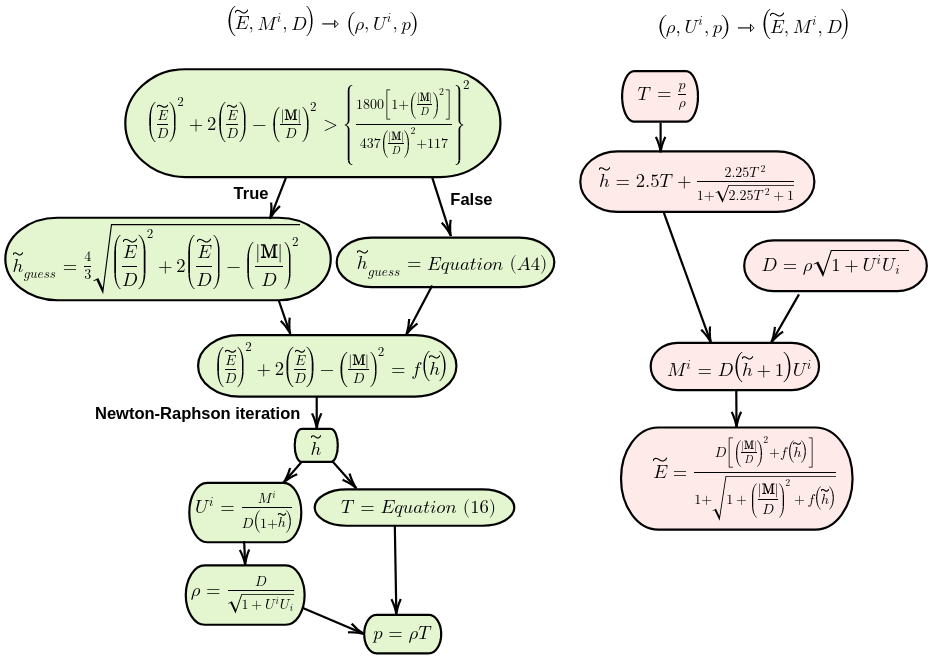
\includegraphics[width=\linewidth]{figures/screenshot.png}
\caption{Flowchart of converting conserved variables to primitive variables (left) and the opposite (right).}
\label{fig:flowchart}
\end{figure}

\definecolor{ErrorURNumerical}{RGB}{1,129,74}
\definecolor{ErrorURExact}{RGB}{224, 201, 73}
\definecolor{ErrorNRNumerical}{RGB}{255,0,0}
\definecolor{ErrorNRExact}{RGB}{0,0,255}
\section{Numerical error analysis for root-finding}
\label{Appendix:Numerical error analysis}
\Cref{fig:flowchart} provides a detailed flowchart of the conversion between primitive and conserved variables. \Cref{fig:ErrorAnalysis} demonstrates that the numerical errors of root-finding arising from the new and original conversion schemes are consistent with the predicted values given by \Cref{eq:ImprovedRelativeError} and \Cref{eq:OriRelativeError}. We measure this conversion error by first converting the input primitive variables $(\rho_0, U^{i}_0, p_0)$ into conserved variables $(D_1, M^{i}_1, \tilde{E}_1)$. Next, we convert $(D_1, M^{i}_1, \tilde{E}_1)$ back to $(\rho_2, U^{i}_2, p_2)$ and then measure the relative error between $\tilde{h}(p_0/\rho_0)\coloneqq\tilde{h}_{0}$ and $\tilde{h}(p_2/\rho_2)\coloneqq\tilde{h}_{2}$. Since the catastrophic cancellation is more prominent in the low-$T$ limit, we measure the error $\abs{1-\tilde{h}_{0}/\tilde{h}_{2}}$ as a function of Mach number from $10^{-4}$ to $10^{6}$ with a fixed non-relativistic temperature $k_{B}T/mc^2=10^{-8}$ (i.e. the blue dashed-dotted line in \Cref{fig:ErrorDistribution}). To verify the accuracy in three-dimensional space, we choose the direction of four-velocity to be parallel to the line $x=y=z$ (i.e. $U^i_0=\abs{\mathbf{U}_0}/\sqrt{3}$ for all $i$). Double precision is adopted to handle the large dynamic range. \Cref{fig:ErrorAnalysis} confirms that the numerical errors of the new and original schemes are mainly caused by round-off errors in the calculation of $\left(\tilde{E}/D\right)^2+2\left(\tilde{E}/D\right)-\left(\abs{\mathbf{M}}/D\right)^2$ and $\left(E/D\right)^2-\left(\abs{\mathbf{M}}/D\right)^2-1$, respectively.




\begin{figure}
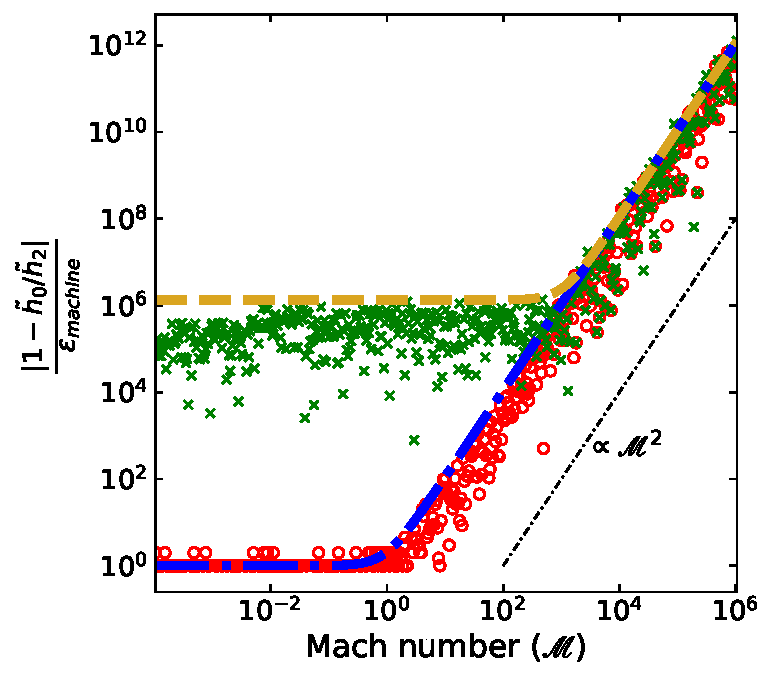
\includegraphics[scale=0.8]{figures/ErrorMap3.pdf}
\caption{Numerical errors of the conversion between primitive and conserved variables. It shows the relative error $\abs{1-\tilde{h}_{0}/\tilde{h}_{2}}$ as a function of Mach number with a given non-relativistic temperature ($k_{B}T/mc^2=10^{-8}$) for the new scheme (red circles) and the original scheme (green crosses). These errors are mainly caused by the cancellation in $\left(\tilde{E}/D\right)^2+2\left(\tilde{E}/D\right)-\left(\abs{\mathbf{M}}/D\right)^2$ and $\left(E/D\right)^2-\left(\abs{\mathbf{M}}/D\right)^2-1$, which are inevitably introduced during the root-finding iteration and consistent with the predicted values given by \Cref{eq:ImprovedRelativeError} (blue dashed-dotted line) and \Cref{eq:OriRelativeError}(brown dashed line).}
\label{fig:ErrorAnalysis}
\end{figure}


\section{Exact solutions of relativistic Riemann problems with the TM equation of state}
\label{appendix:exact solution}
To derive the exact solutions of relativistic Riemann problems with the TM EoS, we have generalized the previous framework of a constant polytropic EoS (\citealt{Marti1994}; \citealt{REZZOLLA2001}) to the TM EoS. More precisely, this approach can be applied to any EoS once we know the relationship between enthalpy and temperature. Here we only summarize the important equations and highlight salient differences from the polytropic EoS. We use the subscripts $L/C_{L}/C_{R}/R$ to refer to the left/left-contact/right-contact/right regions and define the relative four-velocity of $U_{1}$ with respect to $U_{2}$ as $\texttt{Relative}(U_{1}, U_{2})$. Note that we have replaced three-velocity with four-velocity again to avoid catastrophic cancellation in the ultra-relativistic limit.

The exact solution of a relativistic Riemann problem with the TM EoS can be obtained through the following three steps:
\begin{enumerate}
    \item For a given initial condition, we can determine the wave pattern by comparing the relative velocity between the two unperturbed initial states with the three limiting values. These values mark the transition from one wave pattern to another and can be directly computed from the initial condition. See \citet{REZZOLLA2001} for details.
    \item We determine the unknown pressure $p^{*}$ between the left and right waves by numerically solving
    \begin{equation}
    U_{LR}=\texttt{Relative}(U_{LC_{L}}(p^{*}), U_{RC_{R}}(p^{*})),
    \label{eq:p*}
    \end{equation}
    where $U_{LR}=\texttt{Relative}(U_{L}, U_{R})$, $U_{LC_{L}}(p^{*})=\texttt{Relative}(U_{L}, U_{C_{L}}(p^{*}))$, and\\ $U_{RC_{R}}(p^{*})=\texttt{Relative}(U_{R}, U_{C_{R}}(p^{*}))$. Note that the four-velocity in the left-/right-contact region, $U_{C_{L/R}}$, is different for each of the three possible wave patterns. For example, if the left wave is rarefaction and the right wave is shock, then $U_{C_{L}}=U_{\mathscr{R}}(p^*)$ and $U_{C_{R}}=U_{\mathscr{S}}(p^*)$ where $U_{\mathscr{R}}(p^*)$ and $U_{\mathscr{S}}(p^*)$ are defined as follows.
          \begin{enumerate}
          \item $U_{\mathscr{R}}(p^*)$ represents the relation between pressure and flow four-velocity behind the \emph{rarefaction} wave:\\
          Given the pressure behind the rarefaction wave (i.e. $p^{*}$) during the Newton-Raphson iteration for solving \Cref{eq:p*}, we can determine $U_{\mathscr{R}}(p^*)$ by numerically solving the system of equations \eqref{TM EOS}, \eqref{sound_speed}, \eqref{eq:p=rhoT}, \eqref{eq:Riemann invariant}, and \eqref{eq:entropy}:
          \begin{subequations}
          \begin{align}
          &\frac{dU}{d\rho}=\pm \frac{c_{\text{s}}\gamma}{\rho},\label{eq:Riemann invariant}\\
          &\frac{p}{\rho^{5/3}}(h-T)=\text{constant}.\label{eq:entropy}
          \end{align}
          \label{eq: U behind r wave}
          \end{subequations}
          Hereafter, the upper/lower sign applies to the right/left wave. The ordinary differential equation \eqref{eq:Riemann invariant}, known as the Riemann invariant \citep{Rezzolla2018}, relates the dynamical ($U$) and thermal ($c_{\text{s}}$) quantities. \Cref{eq:entropy}, derived from \Cref{TM EOS} and the second law of thermodynamics, results from the fact that entropy is constant through the rarefaction wave. The `constant' in \Cref{eq:entropy} is a function of entropy and can be determined by the thermal quantities in the region unperturbed by the rarefaction wave. In the case of the constant polytropic EoS, \Cref{eq:entropy} reduces to a familiar form: $p/\rho^{\Gamma}=\text{const}$.

          \item $U_{\mathscr{S}}(p^*)$ represents the relation between pressure and flow four-velocity behind the \emph{shock} wave:\\
          Let `up/down' denote the upstream/downstream state of the shock wave. Under the condition that $p_{\text{down}}$ ($p_{\text{down}}=p^{*}$ in this case) is given during the Newton-Raphson iteration for solving \Cref{eq:p*}, we can compute $h_{\text{down}}$ by numerically solving the jump condition of the enthalpy:
          \begin{equation}
          h^2_{\text{up}}-h^2_{\text{down}}=\left(\frac{h_{\text{down}}}{\rho_{\text{down}}}+\frac{h_{\text{up}}}{\rho_{\text{up}}}\right)\left(p_{\text{up}}-p_{\text{down}}\right).
          \label{eq:TaubAdiabatic}
          \end{equation}
          \Cref{eq:TaubAdiabatic} is known as the Taub adiabat \citep{Taub}, where $\rho_{\text{down}}$ can be eliminated using Equations \eqref{T of h} and \eqref{eq:p=rhoT}. After determining $h_{\text{down}}$ by a root-finding routine, the mass flux across the shock can be calculated by
          \begin{equation} J=\left(\frac{p_{\text{down}}-p_{\text{up}}}{h_{\text{up}}/\rho_{\text{up}}-h_{\text{down}}/\rho_{\text{down}}}\right)^{0.5}.
          \label{eq:mass flux}
          \end{equation}
          The four-velocities of shock and post-shock then follow from
          \begin{equation}
          U_{\text{shock}}=\pm \left(\frac{J}{\rho_{\text{up}}}\right)\sqrt{1+U^2_{\text{up}}}\pm U_{\text{up}}\sqrt{1+\left(\frac{J}{\rho_{\text{up}}}\right)^2},
          \label{eq:Ushock}
          \end{equation}
          and
          \begin{equation}
          U_{\mathscr{S}}(p^{*})=\mp \left(\frac{J}{\rho_{\text{down}}}\right)\sqrt{1+U^2_{\text{shock}}}+U_{\text{shock}}\sqrt{1+\left(\frac{J}{\rho_{\text{down}}}\right)^2},
          \label{eq:Udown}
          \end{equation}
          respectively. Equations \eqref{eq:Ushock} and \eqref{eq:Udown} are essentially the Lorentz boost that takes four-velocity from the shock rest frame to the lab frame. Note that the mass flux $J$ is an invariant under the Lorentz boost in the flow direction.
          \end{enumerate}

    \item Once $p^{*}$ is known, $\rho_{\text{down}}$ follows from Equations \eqref{T of h} and \eqref{eq:p=rhoT}, which in turn allows for computing $U_{\text{down}}$ and $U_{\text{shock}}$ through \Cref{eq:Ushock} and \Cref{eq:Udown}. On the other hand, $\rho$ behind the rarefaction wave follows from solving the system of equations \eqref{TM EOS}, \eqref{eq:p=rhoT}, and \eqref{eq:entropy}. Finally, given the self-similar and isentropic character of the rarefaction wave, $\rho$ and $U$ within the rarefaction fan can be computed by solving the system of equations \eqref{eq:Riemann invariant} and $U(\xi)=\texttt{Relative}(\xi/\sqrt{1-\xi^2},\pm c_{s}/\sqrt{1-c_{s}^2})$, where $\xi=x/t$.
    \end{enumerate}

On the basis of above procedure, we show in \Cref{tb:exact solution} the exact solution of the relativistic Riemann problem given in the last row of Table \ref{tb:IC_RiemannProblems} with the TM EoS at $t=80.0$. The source code is available at\\
(\url{https://github.com/zengbs/ExactSolutionRelativisticRiemannProblem}).

\definecolor{MixedLimitsExact}{RGB}{86, 140, 227}
\begin{table}[]
\scriptsize
\caption{
Exact solution of a relativistic Riemann problem with the TM EoS at $t=80.0$. Columns from left to right give $x$-coordinate, proper mass density, four-velocity, and pressure. The initial condition is given in the last row of Table \ref{tb:IC_RiemannProblems}, with the initial discontinuity at $x=5\times10^{-2}$. The blue solid line in \Cref{fig:non-relativistic shock tube} plots the solution. The exact solution is calculated with double precision and shown in 16 digits to reach machine accuracy. The data are available in the supplement.}
\label{tb:exact solution}
\begin{tabular}{@{}cccc@{}}
\toprule
$x$                             & $\rho$                          & $U_{x}$                          & $p$                             \\ \midrule
\texttt{0.0000000000000000e+00} & \texttt{1.0000000000000000e+02} & \texttt{+1.0000000000000000e-03} & \texttt{1.0000000000000000e-04} \\
\texttt{2.5743971630613077e-02} & \texttt{1.0000000000000000e+02} & \texttt{+1.0000000000000000e-03} & \texttt{1.0000000000000000e-04} \\
\texttt{2.6720534130613077e-02} & \texttt{9.9999999999999986e+01} & \texttt{+1.0000000000000002e-03} & \texttt{1.0000000000000000e-04} \\
\texttt{2.8673659130613080e-02} & \texttt{9.8588362795909134e+01} & \texttt{+1.0183105709873300e-03} & \texttt{9.7658360819209613e-05} \\
\texttt{3.1603346630613080e-02} & \texttt{9.6495914226915929e+01} & \texttt{+1.0457764274335814e-03} & \texttt{9.4228343648087098e-05} \\
\texttt{3.6486159130613087e-02} & \texttt{9.3074657510006034e+01} & \texttt{+1.0915528549894106e-03} & \texttt{8.8726314406083176e-05} \\
\texttt{4.2345534130613087e-02} & \texttt{8.9077088828567909e+01} & \texttt{+1.1464845688462534e-03} & \texttt{8.2466343818876140e-05} \\
\texttt{5.2111159130613087e-02} & \texttt{8.2671707042031258e+01} & \texttt{+1.2380374291888151e-03} & \texttt{7.2821829638494934e-05} \\
\texttt{6.4806471630613094e-02} & \texttt{7.4813960019366874e+01} & \texttt{+1.3570561601099081e-03} & \texttt{6.1655409508574801e-05} \\
\texttt{8.4337721630613108e-02} & \texttt{6.3723430244968533e+01} & \texttt{+1.5401619444173906e-03} & \texttt{4.7188055213551995e-05} \\
\texttt{1.1168147163061304e-01} & \texttt{5.0121316453652021e+01} & \texttt{+1.7965101817141935e-03} & \texttt{3.1625521037347636e-05} \\
\texttt{1.5172053413061287e-01} & \texttt{3.3922515604881056e+01} & \texttt{+2.1718776864619303e-03} & \texttt{1.6499866085321606e-05} \\
\texttt{2.0836115913061276e-01} & \texttt{1.7591444669719621e+01} & \texttt{+2.7028867092515813e-03} & \texttt{5.5229310921865207e-06} \\
\texttt{2.0933772163061276e-01} & \texttt{1.7369735883307754e+01} & \texttt{+2.7120420544404751e-03} & \texttt{5.4074080094554571e-06} \\
\texttt{2.0972078270771960e-01} & \texttt{1.7283280852025452e+01} & \texttt{+2.7156332803617649e-03} & \texttt{5.3626249948767070e-06} \\
\texttt{2.6627329885804002e-01} & \texttt{1.7283280852025452e+01} & \texttt{+2.7156332803617649e-03} & \texttt{5.3626249948767070e-06} \\
\texttt{2.6724986145813656e-01} & \texttt{4.0108528993879889e-10} & \texttt{+2.7156332816129858e-03} & \texttt{5.3626249948767070e-06} \\
\texttt{2.6909288248391281e+01} & \texttt{4.0108528993879889e-10} & \texttt{+2.7156332816129858e-03} & \texttt{5.3626249948767070e-06} \\
\texttt{2.6910264810891281e+01} & \texttt{9.9999999999999998e-13} & \texttt{-1.0000000000000000e+02} & \texttt{1.0000000000000000e-10} \\
\texttt{1.0000000000000000e+02} & \texttt{9.9999999999999998e-13} & \texttt{-1.0000000000000000e+02} & \texttt{1.0000000000000000e-10} \\ \bottomrule
\end{tabular}
\end{table}

